\section{Parts Reference}

In this section we list all the necessary parts for the assembly of the prosthetic hand. The parts are divided in three categories: i) the finger parts, ii) the palm parts and iii) the auxiliary parts. The first category consists of all required parts to build all 5 hand fingers, the second category consists of the main palm parts, i.e., the palm structure and the whiffletree mechanism while the third category contains all required parts for building the Herkulex DRS201 servo base, the thumb mechanism, the tendon routing system and the buttons. 


In the following sections we provide a table for each category, listing all parts, along with the names of their corresponding Solidworks part files, their quantity and usage as well as an indication of whether they can be 3D printed. We also provide a separate table with all parts that can be 3D printed. Finally, to facilitate the identification of each part, we provide images of the models. 

\subsection{Finger Parts}



\begin{table}[h!]
	\centering
	\scalebox{0.87}{
		\begin{tabular}{ | l | l | l |}
			\hline
			\multicolumn{3}{|c|}{\bf{Finger Parts List}} \\
			\hline
			{\bf{Part Name}} & {\bf{Qty}} & {\bf{Description}}\\ \hline
			index & 1 & Index Finger [3D printer] \\ \hline
			middle & 1 & Middle Finger [3D printer] \\ \hline
			ring & 1 & Ring Finger [3D printer] \\ \hline
			pinky & 1 & Pinky Finger [3D printer] \\ \hline
			thumb & 1 & Thumb Finger [3D printer] \\ \hline    	
			tubePIP & 10 & Cotton Swab Tube for PIP [d:2mm, D:2.5mm, L:depending on the finger]  \\ \hline
			tubeMIP & 10 & Cotton Swab Tube for MIP [d:2mm, D:2.5mm, L:depending on the finger]  \\ \hline
			tubeDIP & 10 & Cotton Swab Tube for DIP [d:2mm, D:2.5mm, L:depending on the finger]  \\ \hline
			Joint DIP \& MIP & 5 & Silicone Sheet, 60A Durometer  [(Joint Lengthx16.2x4)mm]\\ \hline
			Joint PIP & 5 & Silicone Sheet, 60A Durometer [(Joint Lengthx16.2x5)mm]\\ \hline
			Dyneema Fishing Line & 1 & Tendon Routing [D:0.4mm, Strength:41.5kg] \\ \hline
			Deformable Spong-like Tape & 1 & [Width:10mm, Thickness:5mm] \\ \hline
			Anti-Slip Tape & 1 & 3M Gripping Material [Width:25mm] \\ \hline
			Self-Adhesive Tape & 1 & 3M Scotch 23 [Width:20mm] \\ \hline
		\end{tabular}
	}
\end{table}

\begin{center}
	\begin{tikzpicture}
	\node [mybox] (box){%
		\begin{tabular}{ c c c c}
		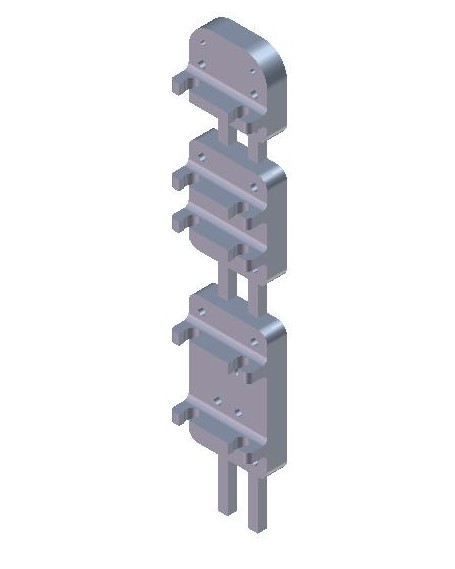
\includegraphics[width=2.8cm]{figures/Parts/index.jpg}   &
		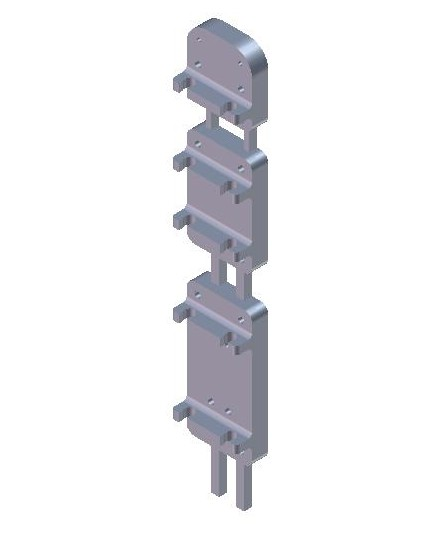
\includegraphics[width=3.0cm]{figures/Parts/middle.jpg}  &
		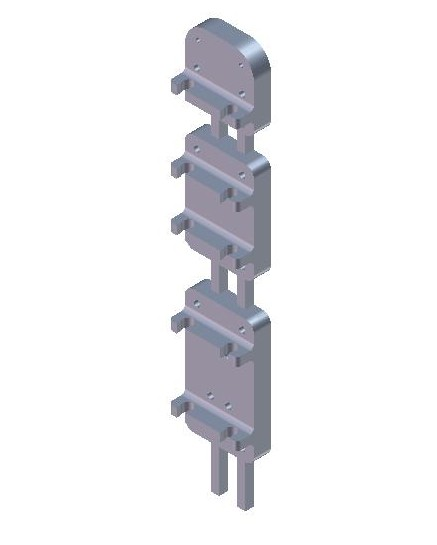
\includegraphics[width=3.0cm]{figures/Parts/ring.jpg}	&
		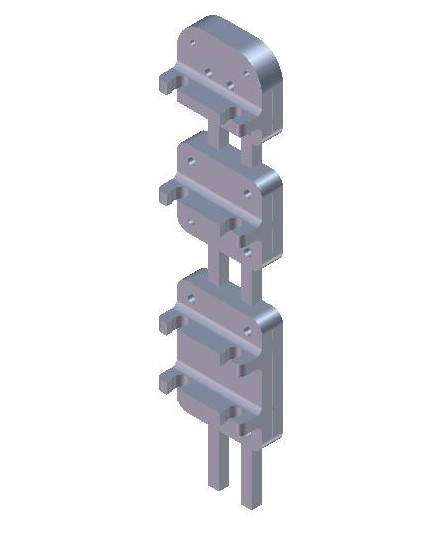
\includegraphics[width=2.7cm]{figures/Parts/pinky.jpg}	\\
		Index &  Middle & Ring & Pinky \\ \\
		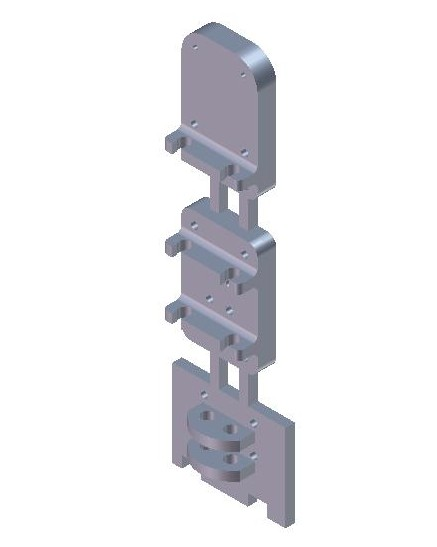
\includegraphics[width=2.7cm]{figures/Parts/thumb.jpg} &
		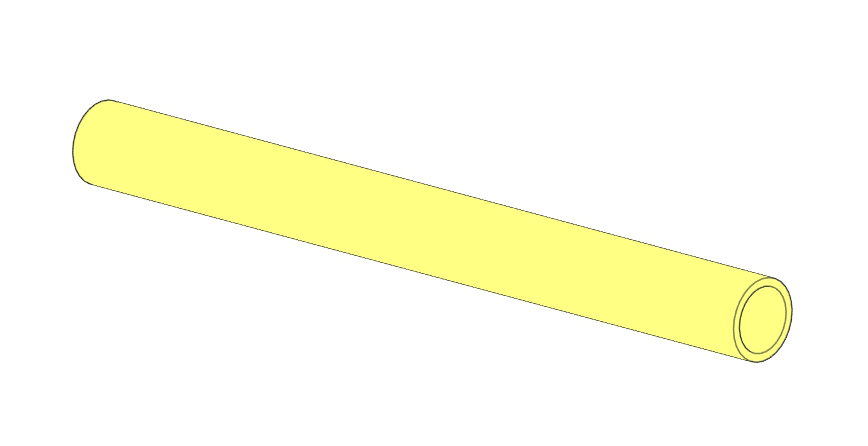
\includegraphics[width=3.0cm]{figures/Parts/Tube.png} &
		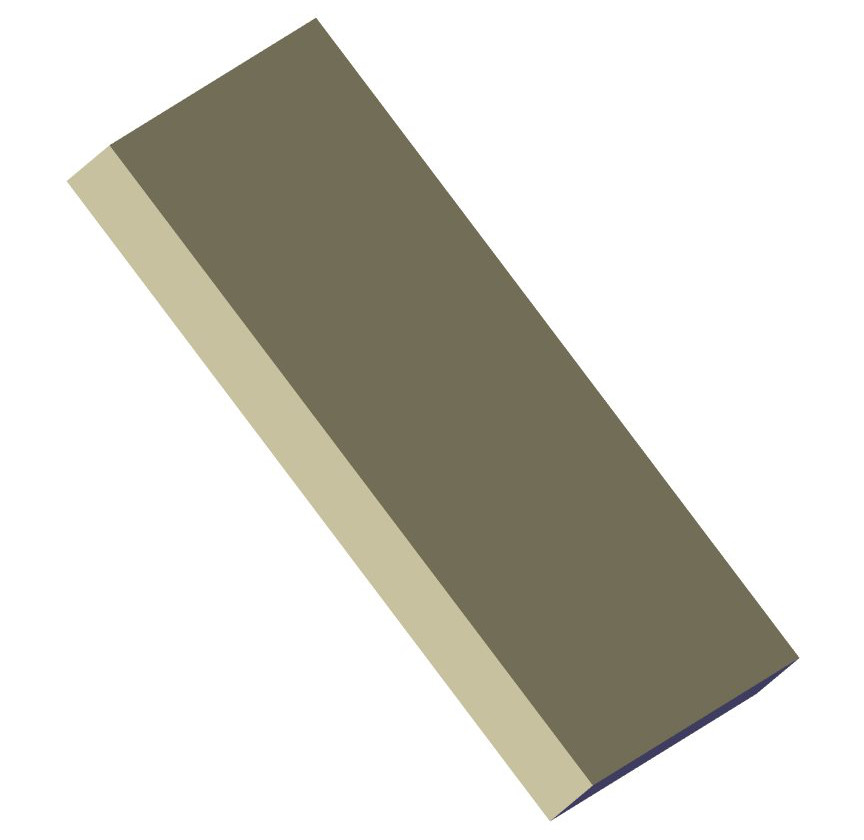
\includegraphics[width=3.0cm]{figures/Parts/SiliconeSheet.jpg} \\
		Thumb & tubes & Joint1, Joint2  \\ \\
		%		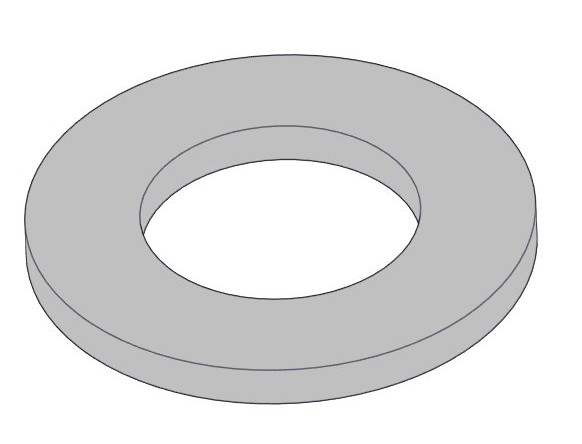
\includegraphics[width=0.9cm]{figures/Parts/WasherM3.jpg} &
		%		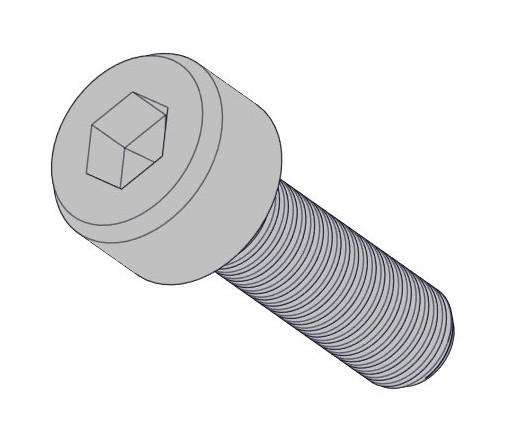
\includegraphics[width=1.8cm]{figures/Parts/ScrewM3x12.jpg} \\		
		%		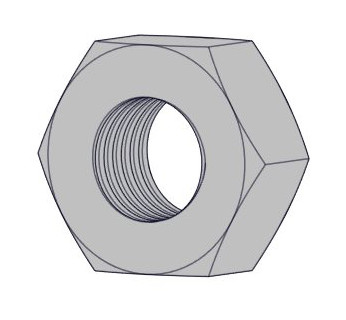
\includegraphics[width=1cm]{figures/Parts/NutM3.jpg} &
		%		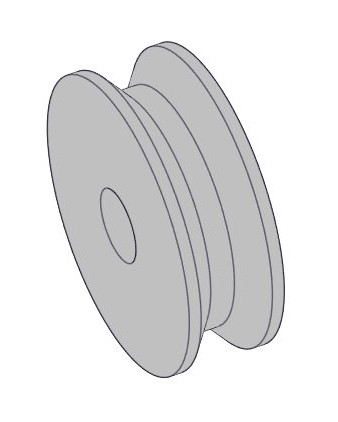
\includegraphics[width=1.4cm]{figures/Parts/Pulley.jpg} \\
		%		M3Nut & pulley  
		\end{tabular}
	};
	\node[mytitle, right=10pt] at (box.north west) {Board 5.1.1: Finger Parts};
	\end{tikzpicture}%
\end{center}

\newpage

\subsection{Palm Parts}


\begin{table}[h!]
	\centering
	\scalebox{0.84}{
		\begin{tabular}{ | l | l | l |}
			\hline
			\multicolumn{3}{|c|}{{\bf{Palm Parts List}}} \\
			\hline
			{\bf{Part Name}} & {\bf{Qty}} & {\bf{Description}}\\ \hline
			palmUp & 1 & Upside of Palm [3D printer] \\ \hline
			PalmDown & 1 & Downside of palm [3D printer] \\ \hline
			barIndexMiddle & 1 & Index \& Middle Fingers Whiphlee Tree Bar [3D printer] \\ \hline
			barRingPinky & 1 & Ring \& Pinky Fingers Whiphlee Tree Bar [3D printer] \\ \hline
			mainBar & 1 & 4 Fingers Whiphlee Tree Bar [3D printer] \\ \hline
			basePulleyInsidePalm & 4 & Tendon Routing of Thumb \& Mount of Base Flange [3D printer] \\ \hline   	    	    	    	
			Dyneema Fishing Line & 1 & Tendon Routing [D:0.4mm, Strength:41.5kg] \\ \hline
			Rubber Foam Tape & 1 & Tape for Palm [Width:10mm, Thickness:4mm] \\ \hline
			Anti-Slip Tape & 1 & 3M Gripping Material [Width:25mm] \\ \hline
			pulley & 1 & V-Groove Sealed Ball Bearing [d:3mm, D:12mm, B:4mm, Deepness:1.2mm] \\ \hline
			PlasticSpacer & 2 & Fastener [d:3.1mm, D:6mm, L:4mm] \\ \hline
			M3X12 Set Screw & 1 & Fastener, M3 Set Screw [L:12mm] \\ \hline	
			M3x16 Socket Cup Screw & 1 & Fastener, M3 Socket Cup Screw [L:16mm] \\ \hline
			M3x20 Socket Cup Screw & 2 & Fastener, M3 Socket Cup Screw [L:20mm] \\ \hline
			M3 Washer & 5 & Fastener, M3 [D:7.5, L:0.5mm] \\ \hline
			M3 Nut & 5 & Fastener, M3 Hex Nut \\ \hline
		\end{tabular}
	}
\end{table}

\vspace{0.2cm}

\begin{center}
	\begin{tikzpicture}
	\node [mybox] (box){%
		\scalebox{0.95}{
		\begin{tabular}{ c c c c }
		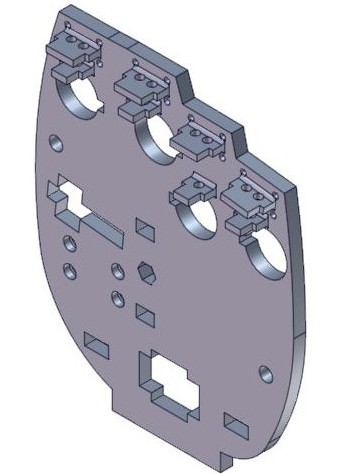
\includegraphics[width=3.5cm]{figures/Parts/palmUp.jpg} &
		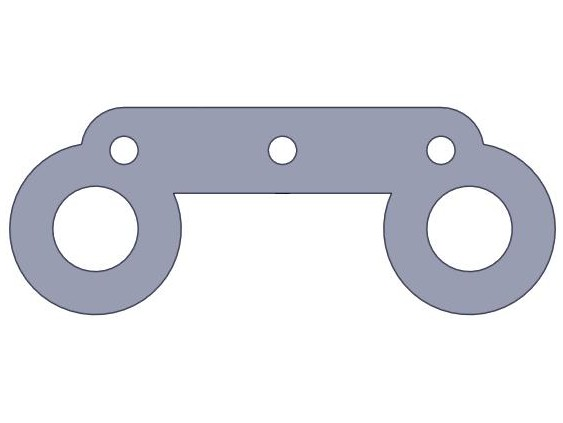
\includegraphics[width=3.2cm]{figures/Parts/barIndexMiddle.jpg} &
		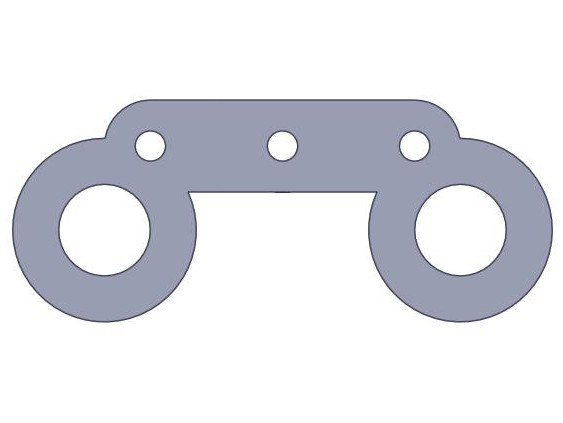
\includegraphics[width=3cm]{figures/Parts/barRingPinky.jpg} & 
		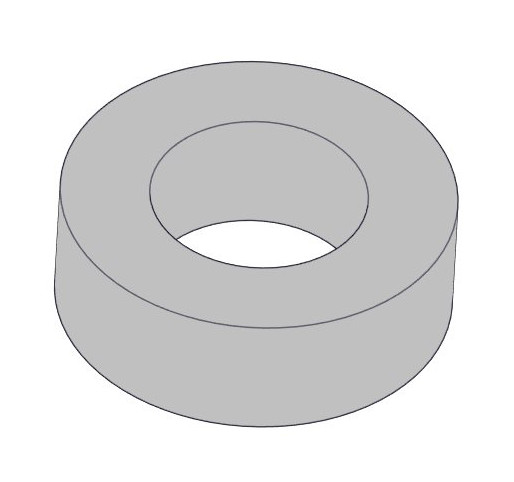
\includegraphics[width=1cm]{figures/Parts/PlasticSpacer.jpg} \\
		palmUp & barIndexMiddle & barRingPinky & PlasticSpacer \\
		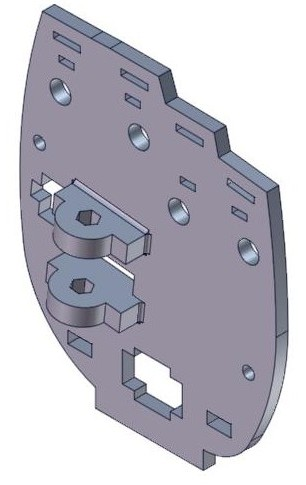
\includegraphics[width=3.3cm]{figures/Parts/palmDown.jpg} &
		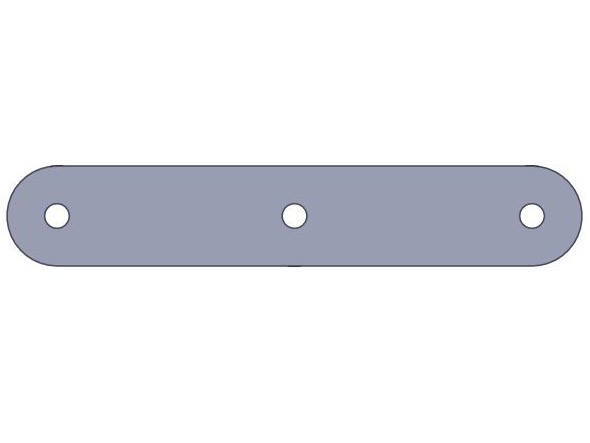
\includegraphics[width=4cm]{figures/Parts/mainBar.jpg} &
		\includegraphics[width=2cm]{figures/Parts/basePulleyInsidePalm.jpg} &
		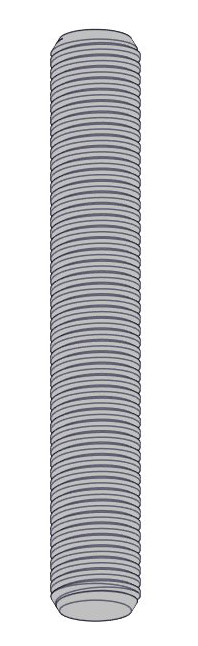
\includegraphics[width=0.9cm]{figures/Parts/M3ThreadRod.jpg} \\
		palmDown & mainBar & basePulleyInsidePalm & M3X12 Set Screw \\
		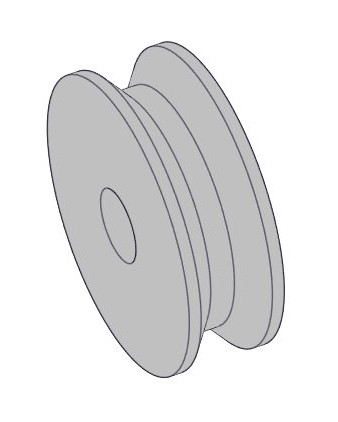
\includegraphics[width=1.4cm]{figures/Parts/Pulley.jpg} &
		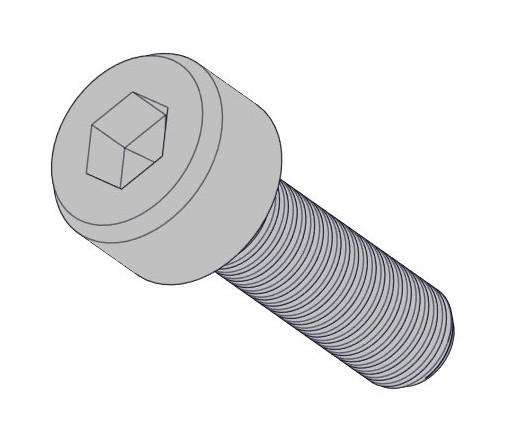
\includegraphics[width=1.8cm]{figures/Parts/ScrewM3x12.jpg} &
		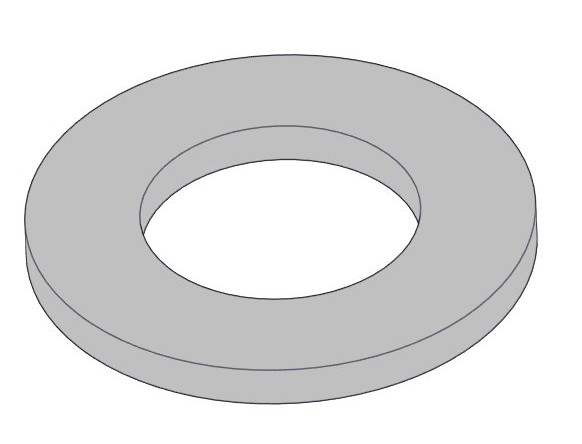
\includegraphics[width=0.9cm]{figures/Parts/WasherM3.jpg} &
		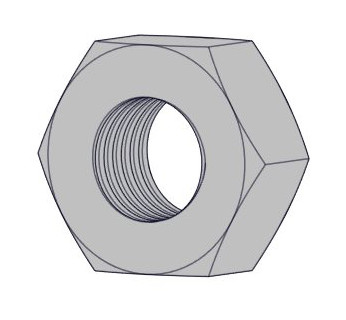
\includegraphics[width=1.4cm]{figures/Parts/NutM3.jpg} \\
		pulley & M3x16, M3x20 & M3 Washer & M3 Nut  \\
		 & Socket Cup Screw & & \\ \\
		\end{tabular}
		}
	};
	\node[mytitle, right=10pt] at (box.north west) {Board 5.2.1: Palm Parts};
	\end{tikzpicture}%
\end{center}

\newpage

\subsection{Auxiliary Parts}

\begin{table}[h!]
	\centering
	\scalebox{0.8}{
		\begin{tabular}{ | l | l | l |}
			\hline
			\multicolumn{3}{|c|}{{\bf{Auxialiary Parts List}}} \\
			\hline
			{\bf{Part Name}} & {\bf{Qty}} & {\bf{Description}}\\ \hline
			baseHerkulex & 1 & Base of HerkuleX DRS201 [3D printer] \\ \hline
			toothedMechanism & 1 & Toothed Mechanism of Base Thumb [3D printer] \\ \hline
			toothedBlockMechanism & 1 & Toothed Block Mechanism of Thumb [3D printer] \\ \hline
			thumbMovingMechanism & 1 & Thumb Moving Mechanism [3D printer] \\ \hline
			thumbButton & 1 & Thumb Base Button [3D printer] \\ \hline
			lockMechanismSupport & 1 & Support of Thumb Lock Mechanism [3D printer] \\ \hline
			lockMechanismBracket & 2 & Bracket of Thumb Lock Mechanism [3D printer] \\ \hline
			pulleyServo & 1 & Pulley of Herkulex DRS201 [3D printer] \\ \hline
			supportPulley1 & 2 & Support pulleys of tendon routing system [3D printer] \\ \hline
			supportPulleyPalmUpAssem & 1 & Support pulley of tendon routing system [3D printer] \\ \hline  	
			dovetailFemale & 1 & Dovetail Female Flange [3D printer] \\ \hline
			flangePlate & 1 & Standard Flange Plate [3D printer] \\ \hline
			buttonBase & 4 & Base of Button [3D printer] \\ \hline    	
			buttonFrame & 4 & Frame of Button [3D printer] \\ \hline 
			buttonAxle & 4 & Axle of Button [3D printer] \\ \hline     	    	    	
			Dyneema & 1 & Tendon Routing [D:0.4mm, Strength:41.5kg] \\ \hline
			HerkulexDRS-201 & 1 & Actuator\\ \hline
			pulley & 4 & V-Groove Sealed Ball Bearing [d:3mm, D:12mm, B:4mm, Deepness:1.2mm] \\ \hline
			
			PlasticSpacer & 4 & Fastener [d:3.1mm, D:6mm, L:4mm] \\ \hline
			M3X18 Set Screw & 3 & Fastener, M3 Set Screw [L:18mm]  \\ \hline	
			M3X30 Set Screw & 1 & Fastener, M3 Set Screw [L:30mm]  \\ \hline	
			M3x6 Socket Cup Screw & 1 & Fastener, M3 Socket Cup Screw [L:6mm] \\ \hline
			M3x10 Socket Cup Screw & 1 & Fastener, M3 Socket Cup Screw [L:10mm] \\ \hline
			M3 Nut & 10 & Fastener, M3 Hex Nut \\ \hline
			M3 Washer & 4 & Fastener, M3 [D:7.5mm, L:0.5mm] \\ \hline
			M2x10 Machine Screw & 4 & Fastener, M2 Machine Screw [L:10mm] \\ \hline
			M2 Nut & 4 & Fastener, M2 Hex Nut \\ \hline
			M2x16 Dowel Pin & 4 & M2 Dowel Pin [L:16mm] \\ \hline
			Compression Spring 6mm L, 9mm OD, 1mm WD & 4 & 9mm Outer Dimension, 1mm Wire Diameter [L:6mm]\\ \hline
		    Compression Spring 3mm L, 3.5mm OD, 0.5mm WD & 1 & 3.5mm Outer Dimension, 0.5mm Wire Diameter [L:3mm]  \\ \hline
		\end{tabular}
	}
\end{table}

\vspace{0.2cm}

\begin{center}
	\begin{tikzpicture}
	\node [mybox] (box){%
		\begin{tabular}{ c c c }
		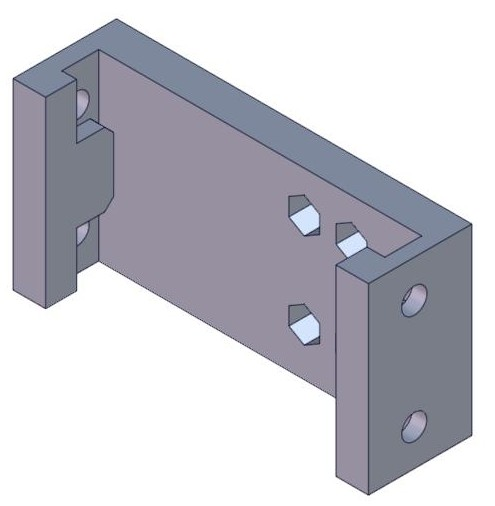
\includegraphics[width=3.1cm]{figures/Parts/baseHerkulex.jpg} &
		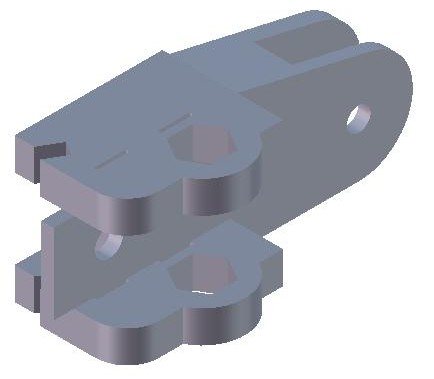
\includegraphics[width=2.7cm]{figures/Parts/thumbMovingMechanism.jpg} &
		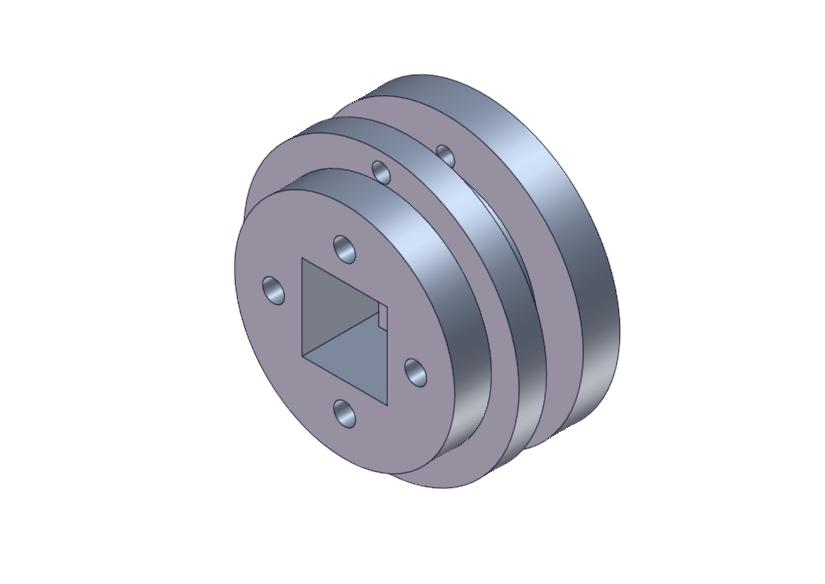
\includegraphics[width=3.3cm]{figures/Parts/pulleyServo.jpg} \\
		baseHerkulex & thumbMovingMechanism & pulleyServo \\
		
\includegraphics[width=3.4cm]{figures/Parts/toothedMechanism.jpg} &
		
\includegraphics[width=1.9cm]{figures/Parts/thumbButton.jpg} & 
		
\includegraphics[width=2.2cm]{figures/Parts/toothedBlockMechanism.jpg} \\
		 toothedMechanism & thumbButton & toothedBlockMechanism  \\
		
\includegraphics[width=2.3cm]{figures/Parts/lockMechanismBracket.jpg} &
		
\includegraphics[width=1.6cm]{figures/Parts/lockMechanismSupport.jpg} \\
		 lockMechanismBracket &  lockMechanismSupport \\
		
		\end{tabular}
	};
	\node[mytitle, right=10pt] at (box.north west) {Board 5.3.1: Auxiliary Parts I};
	\end{tikzpicture}%
\end{center}

\newpage

\begin{center}
	\begin{tikzpicture}
	\node [mybox] (box){%
		\scalebox{0.92}{
		\begin{tabular}{ c c c }
		
\includegraphics[width=2.7cm]{figures/Parts/supportPulley1.jpg} &
		\includegraphics[width=2.7cm]{figures/Parts/supportPulleyPalmUpAssem.jpg} & 
		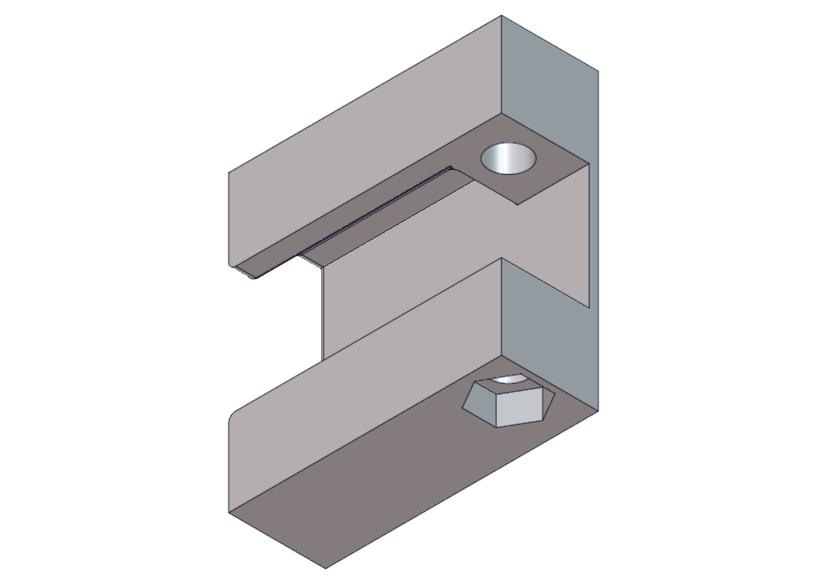
\includegraphics[width=3cm]{figures/Parts/dovetailFemale.jpg} \\
		supportPulley1 & supportPulleyPalmUpAssem & dovetailFemale \\ \\
		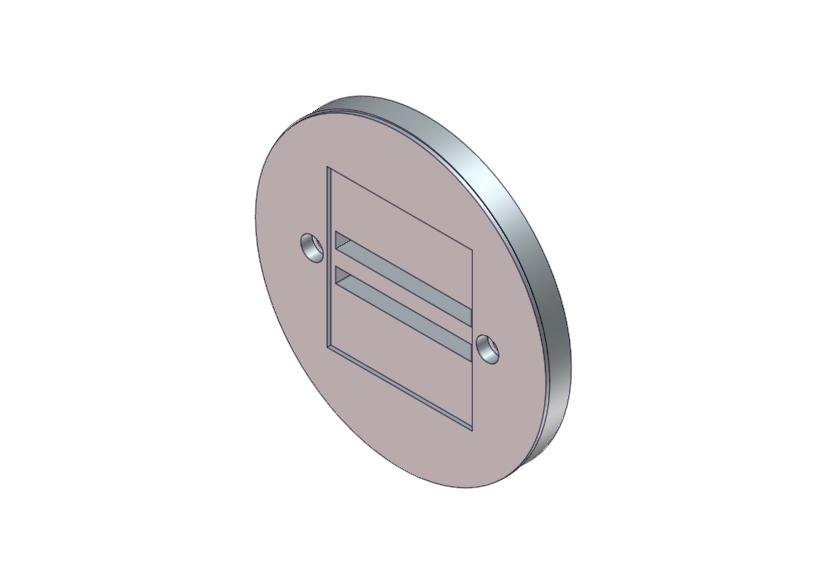
\includegraphics[width=5cm]{figures/Parts/FlangePlate.jpg} &
		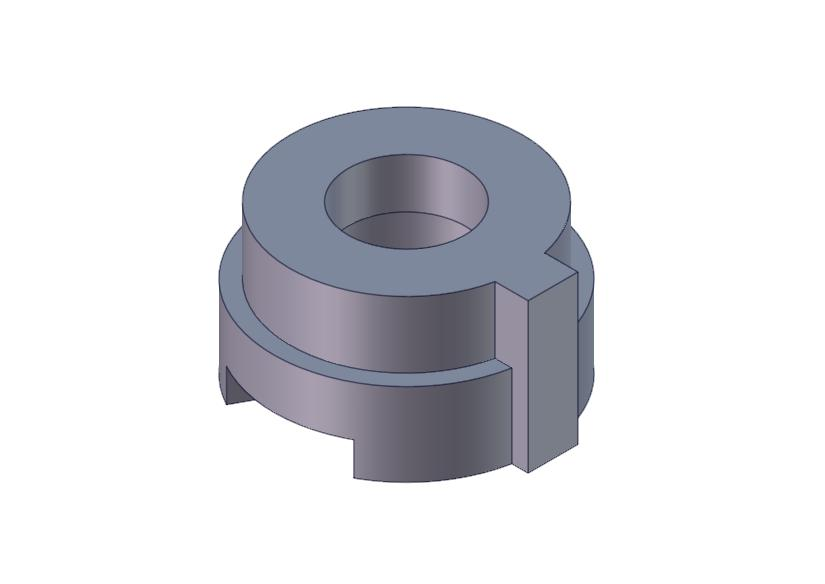
\includegraphics[width=2.1cm]{figures/Parts/buttonBase.jpg} &
		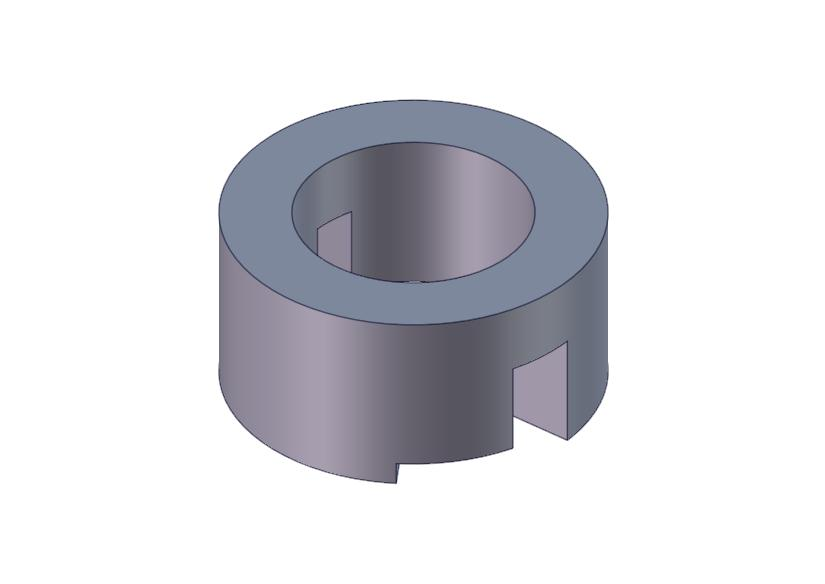
\includegraphics[width=2.1cm]{figures/Parts/buttonFrame.jpg} \\
		flangePlate & buttonBase & buttonFrame \\ \\
		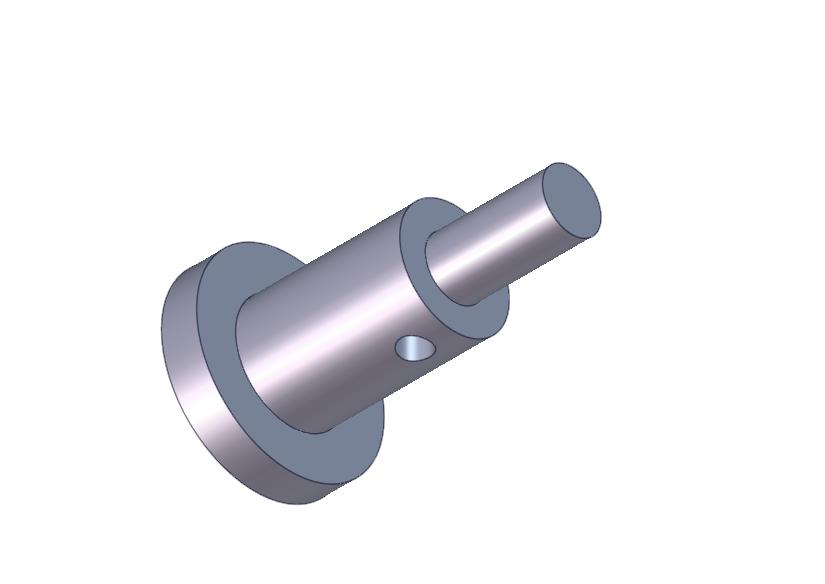
\includegraphics[width=3cm]{figures/Parts/buttonAxle.jpg} &		
		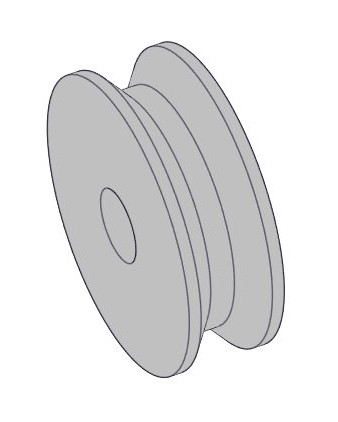
\includegraphics[width=1.4cm]{figures/Parts/Pulley.jpg} &
		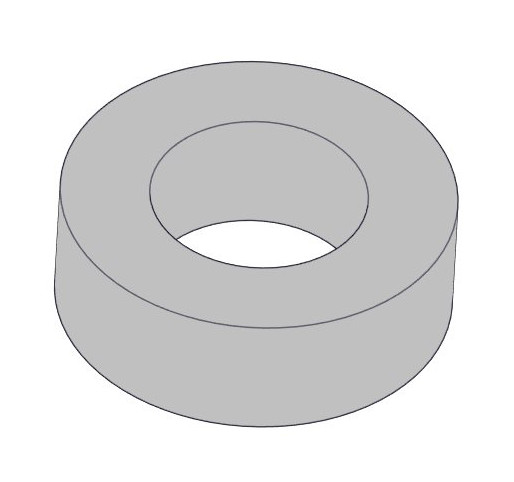
\includegraphics[width=1cm]{figures/Parts/PlasticSpacer.jpg} \\
		buttonAxle & pulley & PlasticSpacer \\ \\
		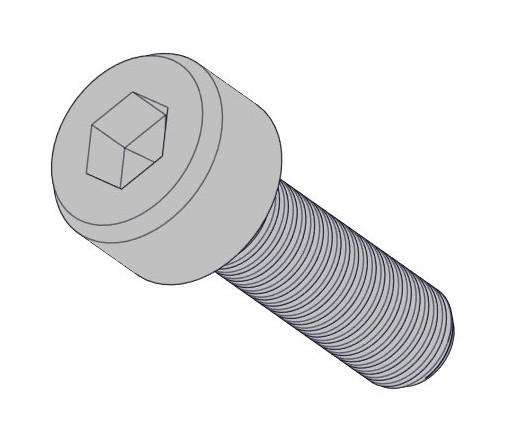
\includegraphics[width=1.8cm]{figures/Parts/ScrewM3x12.jpg} &
		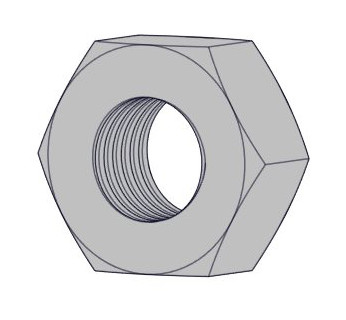
\includegraphics[width=1.4cm]{figures/Parts/NutM3.jpg} &
		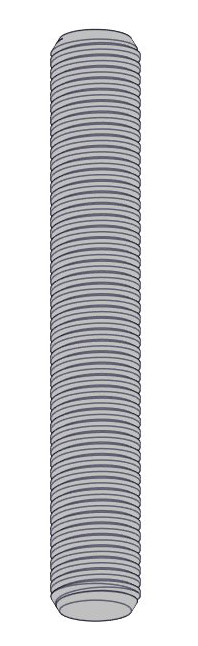
\includegraphics[width=0.9cm]{figures/Parts/M3ThreadRod.jpg} \\
		M3x6, M3x10 & M3 Nut & M3X18, M3X30 \\ 
		Socket Cup Screw & & Set Screw \\ \\
		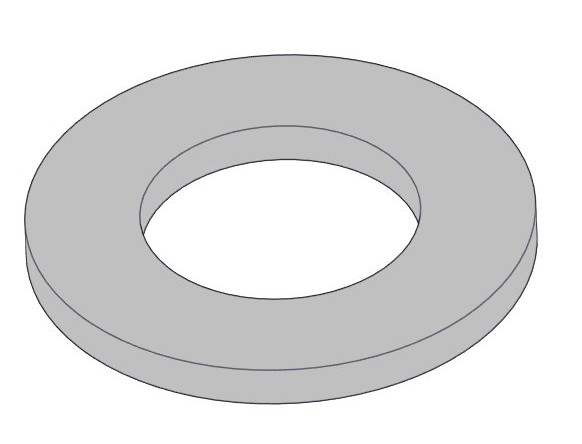
\includegraphics[width=0.9cm]{figures/Parts/WasherM3.jpg} & 
		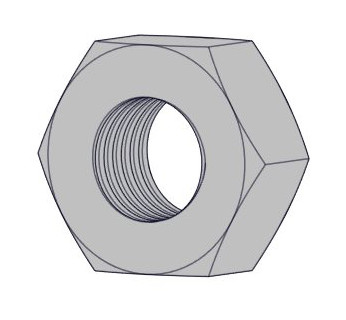
\includegraphics[width=1.2cm]{figures/Parts/NutM3.jpg} &
		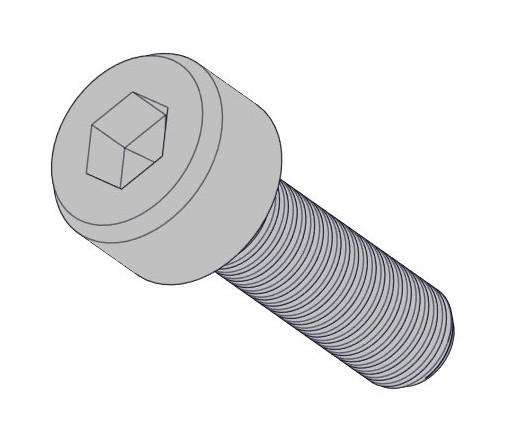
\includegraphics[width=1.6cm]{figures/Parts/ScrewM3x12.jpg} \\
		M3 Washer & M2 Nut & M2x10 Machine Screw \\ \\
		\end{tabular}
		}
	};
	\node[mytitle, right=10pt] at (box.north west) {Board 5.3.2: Auxiliary Parts II};
	\end{tikzpicture}%
\end{center}

\newpage

\subsection{3D Printed Parts}

The following table contains all parts that can be 3D printed. The corresponding STL files contained in the Prosthetic-Hands/CAD directory of our GitHub reporitory (\url{www.github.com/openbionics}) are appropriate to be used with a 3D printer. 


\vspace{0.2cm}

\begin{table}[h!]
	\centering
	\scalebox{0.8}{
		\begin{tabular}{ | l | l | l | l | }
			\hline
			\multicolumn{4}{|c|}{{\bf{3D Printer Parts}}} \\
			\hline
			{\bf{Part Name}} & {\bf{Qty}} & {\bf{Description}} & {\bf{TAZ ABS Profile}}\\ \hline
			index & 1 & Index Finger & Medium, Support Off  \\ \hline
			middle & 1 & Middle Finger & Medium, Support Off \\ \hline
			ring & 1 & Ring Finger & Medium, Support Off \\ \hline
			pinky & 1 & Pinky Finger & Medium, Support Off \\ \hline
			thumb & 1 & Thumb Finger & Medium, Support Off \\ \hline 
			palmUp & 1 & Upside of Palm & Medium, Support On \\ \hline
			PalmDown & 1 & Downside of palm & Medium, Support On \\ \hline
			barIndexMiddle & 1 & Index \& Middle Fingers Whiphlee Tree Bar & Medium, Support Off \\ \hline
			barRingPinky & 1 & Ring \& Pinky Fingers Whiphlee Tree Bar & Medium, Support Off \\ \hline
			mainBar & 1 & 4 Fingers Whiphlee Tree Bar & Medium, Support Off \\ \hline
			basePulleyInsidePalm & 4  & Tendon Routing of Thumb \& Mount of Base Flange & Medium, Support Off \\ \hline
			baseHerkulex & 1 & Base of HerkuleX DRS201 & Medium, Support On \\ \hline
			toothedMechanism & 1 & Toothed Mechanism of Base Thumb & Medium, Support Off \\ \hline
			toothedBlockMechanism & 1 & Toothed Block Mechanism of Thumb & Medium, Support Off \\ \hline
			thumbMovingMechanism & 1 & Thumb Moving Mechanism & Medium, Support On \\ \hline
			thumbButton & 1 & Thumb Base Button & Medium, Support Off \\ \hline
			lockMechanismSupport & 1 & Support of Thumb Lock Mechanism & Medium, Support Off \\ \hline
			lockMechanismBracket & 2 & Bracket of Thumb Lock Mechanism & Medium, Support Off \\ \hline
			pulleyServo & 1 & Pulley of Herkulex DRS201 & Medium, Support On \\ \hline
			supportPulley1 & 2 & Support pulleys of tendon routing system & Medium, Support Off \\ \hline
			supportPulleyPalmUpAssem & 1 & Support pulley of tendon routing system & Medium, Support On \\ \hline  	
			dovetailFemale & 1 & Dovetail Female Flange & Medium, Support On \\ \hline
			flangePlate & 1 & Standard Flange Plate & Medium, Support On \\ \hline
			buttonBase & 4 & Base of Button & Medium, Support On \\ \hline    	
			buttonFrame & 4 & Frame of Button & Medium, Support On \\ \hline 
			buttonAxle & 4 & Axle of Button & Medium, Support On \\ \hline
		\end{tabular}
	}
\end{table}

\vspace{1cm}

For the replication of the prosthetic hand we use the \href{https://download.lulzbot.com/TAZ/4.0/documentation/2014Q2/manual/TAZ_4_Manual.pdf}{LulzBot TAZ 4 3D Printer} and ABS material. We used the settings of the default TAZ Slic3r profiles which can be found \href{https://www.lulzbot.com/support/taz-slic3r-profiles}{here}, except from a small set of parameters that can be found on the following table.

\vspace{1cm}

\begin{table}[h!]
	\centering
	\scalebox{1}{
		\begin{tabular}{ | l | l |}
			\hline
			\multicolumn{2}{|c|}{{\bf{3D Printer Settings}}} \\ \hline
			{\bf{Parameter}} & {\bf{Value}} \\ \hline
			Infill, Fill Density & 20\% \\ \hline
			Infill, Fill Pattern & Honeycomb \\ \hline
			Seam Position & Random \\ \hline
			Brim, Brim Width & 2 mm \\ \hline
		\end{tabular}
	}
\end{table}

\newpage

\subsection{Before Assembling}

Before starting the assembly, the following steps should be followed: \\  \\
$\bullet$ Smoothen the acrylic parts with sandpaper. \\ \\
$\bullet$ Treat the ABS parts with acetone (e.g. see \href{http://blog.reprap.org/2013/02/vapor-treating-abs-rp-parts.html}{reprap Blog}).\\ \\
$\bullet$ Cut the cotton swabs to the appropriate size (following the parts reference dimensions). \\ \\
$\bullet$ Cut the silicone sheets to the appropriate size (following the parts reference dimensions). \\ \\
$\bullet$ Group the parts according to the parts reference. \\ \\
$\bullet$ Pay increased attention to the steps followed by the following icon: \circled{!}\\ \\
%$\bullet$ Note that the provided models do not have the actual size of the parts.\\ \\

\begin{center}
	\begin{tikzpicture}
	\node [mybox] (box){%
		\begin{tabular}{ c }
		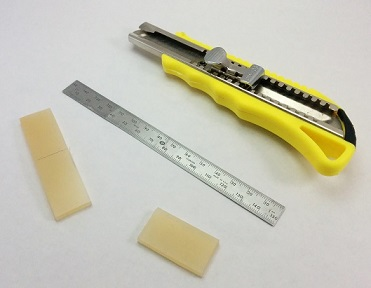
\includegraphics[width=12cm]{figures/Parts/SilliconeCut.jpg} \\
		Cutting the silicone sheets with a cutter and a ruler.
		\end{tabular}
	};
	\node[mytitle, right=10pt] at (box.north west) {Board 5.5.1: Silicone Sheets Preparation};
	\end{tikzpicture}%

\end{center}

